\documentclass[aspectratio=169,10pt]{beamer}

% Theme and Color Scheme
\usetheme{Boadilla}
\usecolortheme{whale}

% Colors
\definecolor{primary}{RGB}{24, 43, 73}       % Deep Navy
\definecolor{secondary}{RGB}{0, 130, 120}    % Deep Teal
\definecolor{accent}{RGB}{233, 84, 32}       % Coral Orange
\definecolor{lightgray}{RGB}{246, 248, 251}  % Clean light gray
\definecolor{darkgray}{RGB}{50, 54, 58}      % Text dark
\definecolor{voidred}{RGB}{210, 40, 30}      % Alert Red

\setbeamercolor{palette primary}{bg=primary,fg=white}
\setbeamercolor{palette secondary}{bg=secondary,fg=white}
\setbeamercolor{palette tertiary}{bg=primary!85!black,fg=white}
\setbeamercolor{structure}{fg=primary}
\setbeamercolor{title}{fg=white,bg=primary}
\setbeamercolor{frametitle}{fg=white,bg=primary}
\setbeamercolor{block title}{bg=primary,fg=white}
\setbeamercolor{block body}{bg=lightgray,fg=darkgray}
\setbeamercolor{block title alerted}{bg=voidred,fg=white}
\setbeamercolor{block body alerted}{bg=voidred!10,fg=darkgray}
\setbeamercolor{block title example}{bg=secondary,fg=white}
\setbeamercolor{block body example}{bg=secondary!10,fg=darkgray}

% Packages
\usepackage{amsmath,amssymb}
\usepackage{booktabs}
\usepackage{tabularx}
\usepackage{tikz}
\usetikzlibrary{shapes,arrows.meta,positioning,calc,fit,backgrounds}
\usepackage{listings}

\lstset{
  basicstyle=\ttfamily\tiny,
  keywordstyle=\color{primary}\bfseries,
  commentstyle=\color{gray},
  stringstyle=\color{accent},
  breaklines=true,
  frame=single,
  backgroundcolor=\color{lightgray}
}

% Title & Author
\title[Greedy Routing in UavNetSim]{\textbf{Comprehensive Analysis of 3D Greedy Forwarding}}
\subtitle{Architecture, Algorithms, and Implementation in UavNetSim}
\author[FANET Research]{UAV Network Simulation Platform}
\institute[CSE Department]{Department of Computer Science and Engineering}
\date{\today}

\begin{document}

% -----------------------------------------------------------------------------
% Slide 1: Title Slide
% -----------------------------------------------------------------------------
\begin{frame}
  \titlepage
\end{frame}

% -----------------------------------------------------------------------------
% Slide 2: Table of Contents
% -----------------------------------------------------------------------------
\begin{frame}{Presentation Outline}
  \tableofcontents
\end{frame}

% =============================================================================
\section{Introduction \& Problem Context}
% =============================================================================

% -----------------------------------------------------------------------------
% Slide 3: Motivation in Flying Ad-hoc Networks (FANETs)
% -----------------------------------------------------------------------------
\begin{frame}{UAV Networks (FANETs) and Routing Challenges}
  \begin{columns}[T]
    \begin{column}{0.52\textwidth}
      \textbf{Why FANET Routing is Challenging:}
      \begin{itemize}\setlength{\itemsep}{0.4em}
        \item \textbf{High 3D Mobility:} Drones move rapidly in $(x, y, z)$ space with dynamic speeds and altitudes.
        \item \textbf{Frequent Link Disruption:} End-to-end paths break within fractions of a second.
        \item \textbf{Resource Scarcity:} On-board energy, queue buffers, and radio channel bandwidth are constrained.
        \item \textbf{Flooding Overhead:} Traditional protocols (AODV, OLSR) flood route discoveries, causing network congestion.
      \end{itemize}
    \end{column}
    \begin{column}{0.45\textwidth}
      \begin{block}{Why Geographic (Greedy) Routing?}
        \begin{itemize}\setlength{\itemsep}{0.4em}
          \item \textbf{Stateless Operation:} Nodes do not maintain full network topology.
          \item \textbf{Strictly Local Decisions:} Each forwarding decision only requires 1-hop neighbor coordinates.
          \item \textbf{Zero Route Discovery Delay:} Packets are transmitted immediately without path establishment latency.
        \end{itemize}
      \end{block}
    \end{column}
  \end{columns}
\end{frame}

% =============================================================================
\section{Theoretical Foundations of Greedy Routing}
% =============================================================================

% -----------------------------------------------------------------------------
% Slide 4: Core Geographic Principle (Corrected spacing & scaled diagram)
% -----------------------------------------------------------------------------
\begin{frame}{The Core Principle: Greedy Distance Minimization}
  \begin{columns}[T]
    \begin{column}{0.48\textwidth}
      \textbf{Mathematical Formulation in 3D Space:}
      \begin{itemize}\setlength{\itemsep}{0.25em}
        \item Current node position: $\mathbf{P}_i = (x_i, y_i, z_i)$
        \item Destination position: $\mathbf{P}_D = (x_D, y_D, z_D)$
        \item 1-hop active neighbors of node $i$: $\mathcal{N}_i$
      \end{itemize}

      \vspace{0.3em}
      \textbf{3D Euclidean Distance Function:}
      \begin{equation*}
        d(\mathbf{P}_A, \mathbf{P}_B) = \sqrt{\Delta x^2 + \Delta y^2 + \Delta z^2}
      \end{equation*}

      \vspace{0.1em}
      \textbf{Greedy Choice Rule:}
      \begin{equation*}
        N^* = \arg\min_{j \in \mathcal{N}_i} d(\mathbf{P}_j, \mathbf{P}_D)
      \end{equation*}

      \textbf{Strict Progress Condition:}
      \begin{equation*}
        d(\mathbf{P}_{N^*}, \mathbf{P}_D) < d(\mathbf{P}_i, \mathbf{P}_D)
      \end{equation*}
    \end{column}

    \begin{column}{0.50\textwidth}
      \centering
      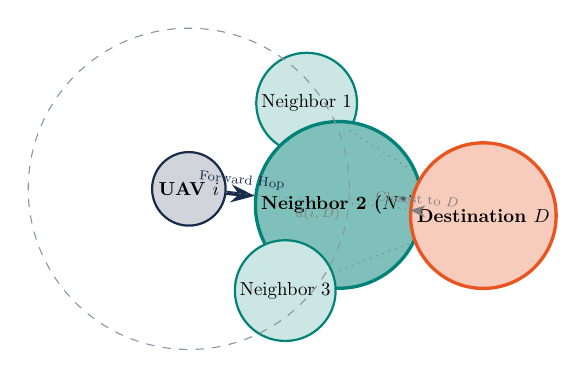
\begin{tikzpicture}[scale=0.68, every node/.style={transform shape}]
        % Drones
        \node[circle, draw=primary, fill=primary!20, thick, inner sep=2.5pt] (Current) at (0, 1.5) {\textbf{UAV $i$}};
        \node[circle, draw=secondary, fill=secondary!20, thick, inner sep=2pt] (N1) at (2.2, 3.1) {Neighbor 1};
        \node[circle, draw=secondary, fill=secondary!50, very thick, inner sep=2.5pt] (Best) at (2.8, 1.2) {\textbf{Neighbor 2 ($N^*$)}};
        \node[circle, draw=secondary, fill=secondary!20, thick, inner sep=2pt] (N3) at (1.8, -0.4) {Neighbor 3};
        \node[circle, draw=accent, fill=accent!30, very thick, inner sep=3pt] (Dst) at (5.5, 1.0) {\textbf{Destination $D$}};

        % Communication range circle
        \draw[dashed, primary!50] (Current) circle (3.0cm);

        % Transmission arrow
        \draw[-{Stealth[length=3mm]}, primary, line width=1.5pt] (Current) -- (Best) node[midway, above, sloped] {\scriptsize Forward Hop};
        \draw[-{Stealth[length=2mm]}, gray, dashed] (Best) -- (Dst) node[midway, above, sloped] {\scriptsize Closest to $D$};
        \draw[gray, dotted] (Current) -- (Dst) node[midway, below] {\scriptsize $d(i, D)$};
        \draw[gray, dotted] (N1) -- (Dst);
        \draw[gray, dotted] (N3) -- (Dst);
      \end{tikzpicture}
      \vspace{0.2em}
      \scriptsize\textit{Figure: Forwarding packet to neighbor closest to destination.}
    \end{column}
  \end{columns}
\end{frame}

% =============================================================================
\section{Greedy Routing Implementation in UavNetSim}
% =============================================================================

% -----------------------------------------------------------------------------
% Slide 5: Codebase Architecture & Components (Clean wrapped layout)
% -----------------------------------------------------------------------------
\begin{frame}{Architecture in UavNetSim}
  The Greedy protocol in \texttt{UavNetSim} is cleanly modularized into three key components:

  \vspace{0.5em}
  \begin{columns}[T]
    \begin{column}{0.31\textwidth}
      \begin{block}{\texttt{GreedyHelloPacket}}
        \scriptsize
        \textbf{File:} \texttt{greedy\_packet.py}
        \begin{itemize}\setlength{\itemsep}{0.3em}
          \item Broadcast beacon packet.
          \item Transmits sender ID and current 3D coords: \texttt{coords}.
          \item Carries creation time for freshness verification.
        \end{itemize}
      \end{block}
    \end{column}

    \begin{column}{0.34\textwidth}
      \begin{block}{\texttt{GreedyNeighborTable}}
        \scriptsize
        \textbf{File:} \texttt{greedy\_neighbor\_table.py}
        \begin{itemize}\setlength{\itemsep}{0.3em}
          \item Inherits from \texttt{BaseTable}.
          \item Stores: \newline \texttt{\{id: [coords, updated\_time]\}}
          \item Enforces entry timeout via \texttt{purge()} ($\tau = 2.0\text{ s}$).
          \item Computes \texttt{best\_neighbor()}.
        \end{itemize}
      \end{block}
    \end{column}

    \begin{column}{0.31\textwidth}
      \begin{block}{\texttt{Greedy}}
        \scriptsize
        \textbf{File:} \texttt{greedy.py}
        \begin{itemize}\setlength{\itemsep}{0.3em}
          \item Main protocol controller.
          \item Manages periodic beaconing with random delay jitter.
          \item Executes \texttt{next\_hop\_selection()}.
          \item Dispatches MAC ACK replies.
          \item Recovers from voids via \texttt{waiting\_list}.
        \end{itemize}
      \end{block}
    \end{column}
  \end{columns}
\end{frame}

% -----------------------------------------------------------------------------
% Slide 6: Neighbor Discovery via Hello Protocol
% -----------------------------------------------------------------------------
\begin{frame}{Component 1: Periodic Neighbor Discovery (Hello Beacons)}
  \begin{columns}[T]
    \begin{column}{0.54\textwidth}
      \textbf{How Drones Discover Each Other:}
      \begin{itemize}\setlength{\itemsep}{0.35em}
        \item Each UAV spawns an asynchronous SimPy process:
          \texttt{broadcast\_hello\_packet\_periodically()}
        \item \textbf{Beacon Interval:} $\Delta t_{\text{hello}} = 0.5\text{ s}$ ($500,000\,\mu\text{s}$)
        \item \textbf{Random Delay Jitter:}
          \begin{equation*}
            \text{jitter} \sim \mathcal{U}(1000\,\mu\text{s}, 2000\,\mu\text{s})
          \end{equation*}
          \textit{Prevents simultaneous broadcasts from colliding on the wireless channel!}
        \item Obtains channel assignment from \texttt{channel\_assigner}.
        \item Queued for broadcast (\texttt{transmission\_mode = 1}).
      \end{itemize}
    \end{column}

    \begin{column}{0.43\textwidth}
      \begin{exampleblock}{Beacon Reception Workflow}
        \small
        When neighbor UAV $j$ receives \texttt{GreedyHelloPacket}:
        \begin{enumerate}\setlength{\itemsep}{0.35em}
          \item Extracts transmitter ID and current 3D position $\mathbf{P}_j$.
          \item Calls \texttt{neighbor\_table.add\_item()}:
            \begin{equation*}
              \text{table}[j] \leftarrow [\mathbf{P}_j, t_{\text{now}}]
            \end{equation*}
          \item No reply or ACK is required for Hello packets.
        \end{enumerate}
      \end{exampleblock}
    \end{column}
  \end{columns}
\end{frame}

% -----------------------------------------------------------------------------
% Slide 7: Neighbor Table Management & Aging (Corrected table formatting)
% -----------------------------------------------------------------------------
\begin{frame}{Component 2: Neighbor Table Aging \& Purging}
  \begin{columns}[T]
    \begin{column}{0.48\textwidth}
      \textbf{The Challenge of High UAV Mobility:}
      \begin{itemize}\setlength{\itemsep}{0.3em}
        \item Drones constantly move in 3D airspace.
        \item If a drone flies away, its cached coordinates become obsolete.
        \item Forwarding to a departed drone causes packet loss.
      \end{itemize}

      \vspace{0.4em}
      \textbf{The Purge Mechanism (\texttt{BaseTable}):}
      \begin{itemize}\setlength{\itemsep}{0.3em}
        \item Entry lifetime: $\tau = 2.0\text{ s}$ ($2\times 10^6\,\mu\text{s}$).
        \item Expired condition:
          \begin{equation*}
            t_{\text{now}} - t_{\text{updated}} > \tau
          \end{equation*}
        \item \texttt{purge()} removes stale nodes before every routing decision!
      \end{itemize}
    \end{column}

    \begin{column}{0.49\textwidth}
      \begin{block}{Data Structure in \texttt{GreedyNeighborTable}}
        \centering
        \scriptsize
        \begin{tabular}{@{}ccc@{}}
          \toprule
          \textbf{Neighbor} & \textbf{3D Coordinates $(x, y, z)$} & \textbf{Status ($t_{\text{now}}=2.5\text{s}$)} \\
          \midrule
          UAV 1 & $(120.4, 85.2, 60.0)$ & Valid ($t=2.1\text{ s}$) \\
          UAV 3 & $(180.1, 140.8, 75.0)$ & Valid ($t=2.3\text{ s}$) \\
          UAV 7 & $(95.6, 210.0, 50.0)$ & \textcolor{voidred}{\textbf{Expired ($t=0.2\text{ s}$)}} \\
          \bottomrule
        \end{tabular}

        \vspace{0.6em}
        \raggedright
        \alert{\textbf{Purge Action:}} UAV 7 is purged because \\
        $(2.5\text{ s} - 0.2\text{ s}) = 2.3\text{ s} > 2.0\text{ s}$.
      \end{block}
    \end{column}
  \end{columns}
\end{frame}

% -----------------------------------------------------------------------------
% Slide 8: Next-Hop Decision Logic (Adjusted vertical height)
% -----------------------------------------------------------------------------
\begin{frame}[fragile]{Component 3: Next-Hop Selection Algorithm}
  \begin{columns}[T]
    \begin{column}{0.48\textwidth}
      \textbf{Algorithm in \texttt{next\_hop\_selection(packet)}:}
      \begin{enumerate}\setlength{\itemsep}{0.25em}
        \item Call \texttt{self.neighbor\_table.purge()}.
        \item Target destination: $\mathbf{P}_D = \texttt{packet.dst\_drone.coords}$.
        \item Set baseline:
          \begin{equation*}
            d^* = d(\mathbf{P}_{\text{self}}, \mathbf{P}_D), \quad \text{best\_id} = \text{self.id}
          \end{equation*}
        \item For each active neighbor $k$ in table:
          \begin{itemize}\setlength{\itemsep}{0.1em}
            \item Compute $d_k = d(\mathbf{P}_k, \mathbf{P}_D)$
            \item If $d_k < d^* \implies d^* \leftarrow d_k, \text{best\_id} \leftarrow k$
          \end{itemize}
        \item \textbf{Decision Evaluation:}
          \begin{itemize}\setlength{\itemsep}{0.1em}
            \item $\text{best\_id} \neq \text{self.id} \implies$ \textbf{\texttt{has\_route = True}}
            \item $\text{best\_id} == \text{self.id} \implies$ \alert{\textbf{\texttt{has\_route = False}}}
          \end{itemize}
      \end{enumerate}
    \end{column}

    \begin{column}{0.49\textwidth}
      \begin{exampleblock}{Python Implementation (\texttt{greedy\_neighbor\_table.py})}
\begin{lstlisting}[language=Python]
def best_neighbor(self, my_drone, dst_drone):
    best_distance = euclidean_distance_3d(
        my_drone.coords, dst_drone.coords)
    best_id = my_drone.identifier

    for key in self.table.keys():
        next_pos = self.table[key][0]
        temp_dist = euclidean_distance_3d(
            next_pos, dst_drone.coords)
        if temp_dist < best_distance:
            best_distance = temp_dist
            best_id = key
            self.have_void_area = 0

    return best_id
\end{lstlisting}
      \end{exampleblock}
    \end{column}
  \end{columns}
\end{frame}

% -----------------------------------------------------------------------------
% Slide 9: Packet Reception, Forwarding & MAC ACK Handshake
% -----------------------------------------------------------------------------
\begin{frame}{Component 4: Reception, Forwarding \& MAC ACK Handshake}
  \begin{columns}[T]
    \begin{column}{0.48\textwidth}
      \textbf{Packet Arrival (\texttt{packet\_reception}):}
      \begin{itemize}\setlength{\itemsep}{0.3em}
        \item \textbf{Case A: Current Node is Destination}
          \begin{itemize}\setlength{\itemsep}{0.15em}
            \item Calculates metrics (E2E delay, throughput).
            \item Generates \texttt{AckPacket} to previous hop.
            \item Waits \texttt{SIFS\_DURATION} ($10\,\mu\text{s}$).
            \item Unicasts ACK directly via physical channel.
          \end{itemize}
        \item \textbf{Case B: Intermediate Relay Node}
          \begin{itemize}\setlength{\itemsep}{0.15em}
            \item Checks \texttt{qsize < max\_queue\_size}.
            \item If space: enqueues packet, returns ACK.
            \item If full: packet is dropped (Buffer Overflow).
          \end{itemize}
      \end{itemize}
    \end{column}

    \begin{column}{0.48\textwidth}
      \begin{block}{MAC Retransmission \& Blocking}
        \begin{itemize}\setlength{\itemsep}{0.3em}
          \item Sender waits for ACK via \texttt{wait\_ack} process.
          \item When \texttt{AckPacket} arrives:
            \begin{itemize}\setlength{\itemsep}{0.15em}
              \item Records MAC delay metric.
              \item Removes packet from transmission queue.
              \item Interrupts waiting process.
            \end{itemize}
          \item Retry limit: \texttt{MAX\_RETRANSMISSION\_ATTEMPT = 5}.
          \item Models realistic CSMA/CA Head-of-Line (HoL) channel contention.
        \end{itemize}
      \end{block}
    \end{column}
  \end{columns}
\end{frame}

% =============================================================================
\section{The Routing Void Problem \& Simulator Solution}
% =============================================================================

% -----------------------------------------------------------------------------
% Slide 10: The Routing Void Problem (Scaled diagram & neat bounds)
% -----------------------------------------------------------------------------
\begin{frame}{The Routing Void (Local Minimum) Problem in 3D}
  \begin{columns}[T]
    \begin{column}{0.48\textwidth}
      \alert{\textbf{What is a 3D Routing Void?}}
      \begin{itemize}\setlength{\itemsep}{0.3em}
        \item Occurs when current drone $i$ is closer to destination $D$ than \textbf{any} neighbor:
          \begin{equation*}
            \forall j \in \mathcal{N}_i, \quad d(\mathbf{P}_j, \mathbf{P}_D) > d(\mathbf{P}_i, \mathbf{P}_D)
          \end{equation*}
        \item Greedy forwarding reaches a dead end: \texttt{has\_route = False}.
        \item \textbf{Causes in 3D UAV Networks:}
          \begin{itemize}\setlength{\itemsep}{0.15em}
            \item Sparse network deployment.
            \item Building obstacles / no-fly zones.
            \item Altitude dispersion separating nodes.
          \end{itemize}
      \end{itemize}
    \end{column}

    \begin{column}{0.50\textwidth}
      \centering
      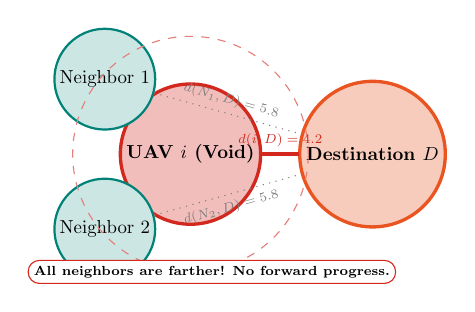
\begin{tikzpicture}[scale=0.68, every node/.style={transform shape}]
        % Drones
        \node[circle, draw=voidred, fill=voidred!30, very thick, inner sep=2.5pt] (Current) at (1.8, 1.5) {\textbf{UAV $i$ (Void)}};
        \node[circle, draw=secondary, fill=secondary!20, thick, inner sep=2pt] (N1) at (0.2, 2.9) {Neighbor 1};
        \node[circle, draw=secondary, fill=secondary!20, thick, inner sep=2pt] (N2) at (0.2, 0.1) {Neighbor 2};
        \node[circle, draw=accent, fill=accent!30, very thick, inner sep=3pt] (Dst) at (5.2, 1.5) {\textbf{Destination $D$}};

        % Range
        \draw[dashed, voidred!60] (Current) circle (2.2cm);

        % Distances
        \draw[voidred, line width=1.2pt] (Current) -- (Dst) node[midway, above] {\scriptsize $d(i, D) = 4.2$};
        \draw[gray, dotted] (N1) -- (Dst) node[midway, above, sloped] {\scriptsize $d(N_1, D) = 5.8$};
        \draw[gray, dotted] (N2) -- (Dst) node[midway, below, sloped] {\scriptsize $d(N_2, D) = 5.8$};

        % Void label
        \node[draw=voidred, fill=white, rounded corners, inner sep=3pt] at (2.2, -0.7) {\scriptsize \alert{\textbf{All neighbors are farther! No forward progress.}}};
      \end{tikzpicture}
    \end{column}
  \end{columns}
\end{frame}

% -----------------------------------------------------------------------------
% Slide 11: Store-and-Carry Void Resolution (Balanced vertical layout)
% -----------------------------------------------------------------------------
\begin{frame}{Store-and-Carry Void Resolution in UavNetSim}
  Unlike 2D networks that use planar face traversal (GPSR perimeter mode), \texttt{UavNetSim} leverages \textbf{UAV Mobility via Store-and-Carry}:

  \vspace{0.4em}
  \begin{columns}[T]
    \begin{column}{0.48\textwidth}
      \begin{block}{The \texttt{waiting\_list} Mechanism}
        \small
        \begin{enumerate}\setlength{\itemsep}{0.3em}
          \item When \texttt{has\_route == False}:
            \begin{itemize}\setlength{\itemsep}{0.15em}
              \item Packet is moved to \texttt{my\_drone.waiting\_list}.
              \item Removed from \texttt{transmitting\_queue}.
            \end{itemize}
          \item Periodic monitoring process runs:
            \texttt{check\_waiting\_list()}
          \item Polling interval: $\Delta t_{\text{check}} = 0.6\text{ s}$ ($600,000\,\mu\text{s}$).
        \end{enumerate}
      \end{block}
    \end{column}

    \begin{column}{0.48\textwidth}
      \begin{block}{Re-Evaluation Lifecycle}
        \small
        On each check interval:
        \begin{enumerate}\setlength{\itemsep}{0.3em}
          \item \textbf{Deadline Verification:}
            \begin{equation*}
              t_{\text{now}} > t_{\text{creation}} + \text{deadline} \implies \text{Drop}
            \end{equation*}
          \item \textbf{Mobility Resolution:}
            UAVs have moved! Re-evaluates \texttt{best\_neighbor(my\_drone, dst)}.
          \item If a neighbor now provides forward progress:
            \begin{itemize}\setlength{\itemsep}{0.15em}
              \item Re-insert packet into \texttt{transmitting\_queue}.
              \item Remove packet from \texttt{waiting\_list}.
            \end{itemize}
        \end{enumerate}
      \end{block}
    \end{column}
  \end{columns}
\end{frame}

% =============================================================================
\section{Protocol Evaluation \& Comparison}
% =============================================================================

% -----------------------------------------------------------------------------
% Slide 12: Strengths & Weaknesses
% -----------------------------------------------------------------------------
\begin{frame}{Strengths \& Limitations of Greedy Routing}
  \begin{columns}[T]
    \begin{column}{0.48\textwidth}
      \begin{exampleblock}{\textbf{Advantages (Pros)}}
        \begin{itemize}\setlength{\itemsep}{0.3em}
          \item \textbf{Minimal Memory Footprint:} Requires only 1-hop neighbor table ($O(k)$ vs $O(N)$).
          \item \textbf{Ultra-low Control Overhead:} No global route discovery; only periodic 1-hop Hello beacons.
          \item \textbf{Zero Path Discovery Latency:} Packets are dispatched immediately if a neighbor exists.
          \item \textbf{Mobility Resilient:} Dynamically makes hop-by-hop decisions without full path repair.
        \end{itemize}
      \end{exampleblock}
    \end{column}

    \begin{column}{0.48\textwidth}
      \begin{alertblock}{\textbf{Disadvantages (Cons)}}
        \begin{itemize}\setlength{\itemsep}{0.3em}
          \item \textbf{Susceptible to Voids:} High latency or packet drops when node density is sparse.
          \item \textbf{Outdated Coordinates:} High speeds ($10\text{--}30\text{ m/s}$) can render reported beacon positions stale.
          \item \textbf{Channel Unaware:} Only measures distance; ignores fading, interference, and SINR!
        \end{itemize}
      \end{alertblock}
    \end{column}
  \end{columns}
\end{frame}

% -----------------------------------------------------------------------------
% Slide 13: Comparison with Other Protocols (Fitted table, no overflow)
% -----------------------------------------------------------------------------
\begin{frame}{Comparison with Other Protocols in UavNetSim}
  \centering
  \resizebox{0.95\textwidth}{!}{%
    \begin{tabular}{lcccc}
      \toprule
      \textbf{Routing Protocol} & \textbf{Routing Paradigm} & \textbf{Metric Used} & \textbf{Control Overhead} & \textbf{Void Resilience} \\
      \midrule
      \textbf{Greedy} & Geographic & 3D Euclidean Distance & Very Low (1-hop) & Moderate (Store/Carry) \\
      \textbf{DSDV} & Proactive Table & Hop Count & High (Table Flooding) & Low in high mobility \\
      \textbf{GRAD} & Gradient-based & Hop gradient + energy & Low & High \\
      \textbf{OPAR} & Position + Predictive & Position + Velocity & Medium & High \\
      \textbf{Q-Routing / QMR} & Reinforcement Learning & Q-value (Delay / SINR / Energy) & Low-Medium & Very High (Adaptive) \\
      \bottomrule
    \end{tabular}%
  }

  \vspace{0.8em}
  \begin{block}{Key Takeaway}
    Greedy Routing serves as the \textbf{foundational geographic baseline} in \texttt{UavNetSim}. Advanced protocols like \textbf{QMR} and \textbf{OPAR} build on top of geographic forwarding by integrating channel SINR, residual energy, and reinforcement learning reward metrics.
  \end{block}
\end{frame}

% -----------------------------------------------------------------------------
% Slide 14: Conclusion & Key Takeaways
% -----------------------------------------------------------------------------
\begin{frame}{Summary \& Conclusions}
  \begin{itemize}\setlength{\itemsep}{0.4em}
    \item \textbf{Role in UavNetSim:} Serves as the primary geographic routing benchmark for UAV ad-hoc networking research.
    \item \textbf{Simplicity \& Efficiency:} Relies strictly on 1-hop periodic Hello beacons ($0.5\text{ s} + \text{jitter}$) and 3D Euclidean distance calculations.
    \item \textbf{Dynamic Table Maintenance:} Purging mechanism with a $2.0\text{ s}$ timeout ensures that stale coordinates are eliminated before decisions are made.
    \item \textbf{Handling Routing Voids:} Utilizes a store-and-carry \texttt{waiting\_list} polled every $0.6\text{ s}$, relying on UAV mobility to resolve dead-ends without packet loss.
    \item \textbf{Future Enhancements:} Can be combined with channel-aware metrics (SINR/fading from Sionna RT) or Q-Learning for multi-criteria next-hop optimization.
  \end{itemize}
\end{frame}

% -----------------------------------------------------------------------------
% Slide 15: Q&A
% -----------------------------------------------------------------------------
\begin{frame}
  \begin{center}
    \Huge \textbf{\textcolor{primary}{Thank You!}}

    \vspace{1.0em}
    \Large \textbf{\textcolor{secondary}{Questions \& Discussion}}

    \vspace{1.5em}
    \normalsize
    \textbf{Project:} UavNetSim (Autonomous UAV Network Simulation Platform) \\
    \textit{Source code verified in} \texttt{routing/greedy/}
  \end{center}
\end{frame}

\end{document}
